\subsection{Image Classification}


\subsection{QA System}

\begin{table}[!t]
\vspace{-5pt}
\small
\vspace{7pt}
\caption{QA System performance based on optimizers (SGD, Adam, LARS, LAMB) across different batch sizes (64, 128, 256, 512).}\label{tbl:results}
\vspace{-10pt}
\begin{center}
\begin{tabular}{ c|c|c|c|c}
\multicolumn{1}{c|}{} &  \multicolumn{4}{c}{Batch Size}\\ \cline{2-5}
\multicolumn{1}{c|}{Optimizer} &
 \multicolumn{1}{c|}{64} &
 \multicolumn{1}{c|}{128} &
 \multicolumn{1}{c|}{256} &
 \multicolumn{1}{c}{512} \\
 %& & \\
\hline
SGD & 4.76 & 5.00 & 5.38 & 6.45\\
Adam &  4.59 & \cellcolor{gray!30} 4.59 &  \cellcolor{gray!30} 4.49 & \cellcolor{gray!30} 4.53\\
LARS & 8.36 & 8.42 & 8.57 & 9.43\\
LAMB & \cellcolor{gray!30} 4.58 & 4.62 & 4.59 & 4.86\\
\end{tabular}
\end{center}
\vspace{-15pt}
\end{table}

\begin{figure}[!t]
    \centering
    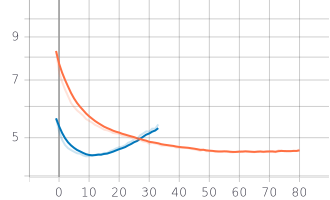
\includegraphics[width=0.7\linewidth]{img/adam_blue_lamb_orange_drqa_256.png}
    \caption{Adam (light blue) and LAMB (orange) test loss convergence graph with batch size of 256.}
    \label{fig:256}
\end{figure}

\begin{figure}[!t]
    \centering
    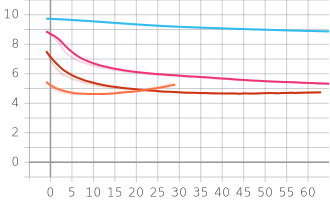
\includegraphics[width=0.7\linewidth]{img/drqa_128_blars_oadam_psgd_rlamb.png}
    \caption{LARS (light blue), SGD (pink), LAMB (red), and Adam (orange) test loss convergence graph.}
    \label{fig:128}
\end{figure}

The experimentation is conducted by deploying the model from \S\ref{sec:method}.B against the dedicated four optimizers in this study (SGD, Adam, LARS, and LAMB) across various batch sizes (64, 128, 256, 512). The results are reported in the Table~\ref{tbl:qasystem}. The gray cells denote the winner (the one with the lowest loss overall test loss values in the same column) across each batch size. The results were surprising as LAMB only outperformed Adam in a batch size of 64 but lost in the other batch sizes. LARS performed the worst across every run, where it was bested by traditional SGD consistently. Moreover, as the batch size increased, the gap between performances increased. This contradicts what has been observed in current literature \cite{}. We did not observe the performance increase of the QA system with larger batch sizes across the layer-wise adaptive techniques. However, there are two possible explanations for these results, which include: 
\begin{itemize}
    \item The batch sizes tested in the QA system were statistically small in comparison to most literature (which reported sizes of 4K or >8K)
    \item Based on Figure \ref{fig:256}, Adam over-fitted a lot more quickly and triggered the early stop procedure, while the other algorithms did not. A similar trend can be observed in Figure \ref{fig:128} where LAMB converged very slowly and it can easily be deduced that a longer training time would allow for an even lower test loss value (and higher overall accuracy) than ADAM ever could reach
\end{itemize}

\subsection{Speech-to-Text}

